
\section{Conditionneur simple}
\subsection{Principe de mesure}

Le principe de mesure consiste en une source de tension qui alimente un pont diviseur
de tension avec une résistance fixe \(R1\) et une autre représentant le capteur \(Rc\).

\begin{figure}[H]
    \centering
    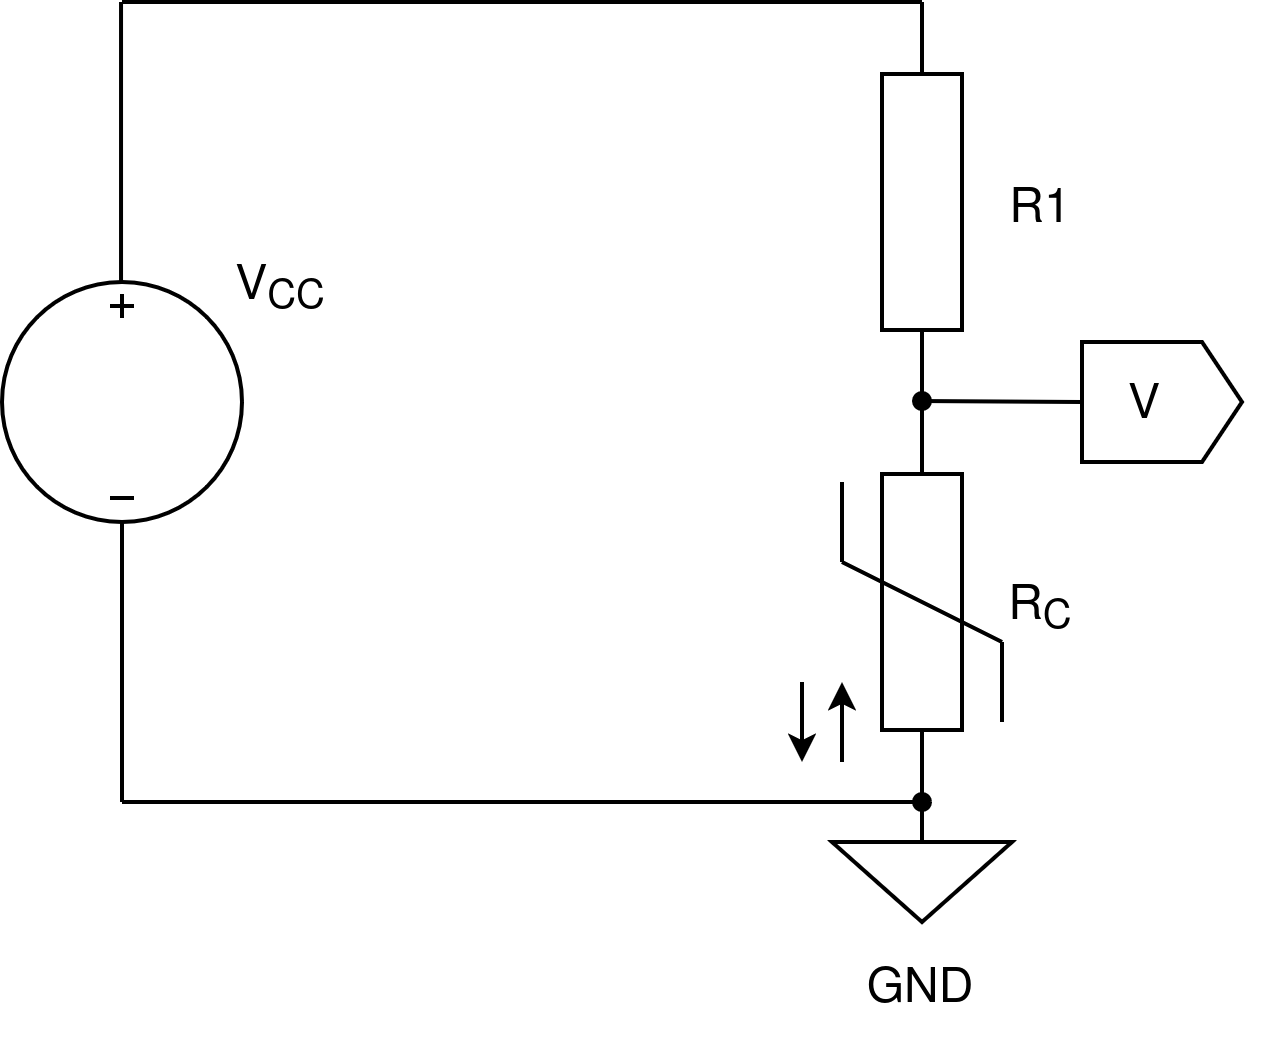
\includegraphics[width=0.5\textwidth]{pont-div}
    \caption{Conditionneur simple}
    \label{fig:conditionneur}
\end{figure}

Le montage suivant nous permet d’écrire la tension \(V\) :
\[
    V=\frac{R_c}{R_1+R_c}V_{cc}
\]

L’évolution de \(V\) en fonction de \(R_c\) n’est pas linéaire :
\[
    \frac{V}{V_{cc}}=\frac{x}{1+x}\quad\text{avec}\ x=\frac{R_c}{R_1}
\]

\begin{figure}[H]
    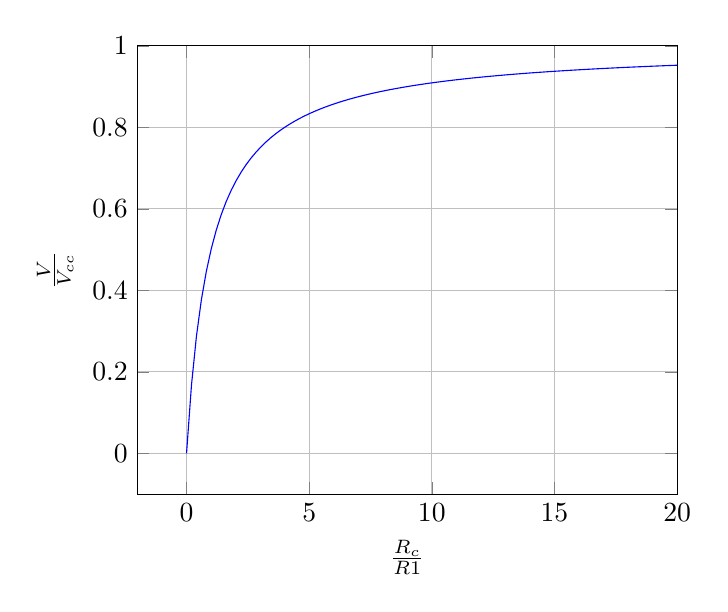
\begin{tikzpicture}
        \begin{axis}[
            xmax=20,
            ymax=1,
            xlabel=\(\frac{R_c}{R1}\),
            ylabel=\(\frac{V}{V_{cc}}\),
            grid=both,
        ]
            \addplot[domain=0:20, samples=100, color=blue]{x/(1+x)};
        \end{axis}
    \end{tikzpicture}
    \caption{Trace de la fonction \(\frac{V}{V_{cc}}=\frac{R_c}{R_1+R_c}\)}
    \label{fig:cond-simple}
\end{figure}

\subsection{Choix de la valeur de \(R1\)}

Considérons un conditionneur de signal basé sur un pont diviseur résistif 
alimenté par une tension \( V_{cc} \), et composé de deux résistances : 
\( R_1 = R_0 \) (fixe), et \( R_c = R_0 + \Delta R \), une résistance variable 
représentant le capteur.

La tension de sortie \( V \) prélevée au point milieu du diviseur s’écrit :
\[
V = \frac{R_c}{R_1 + R_c} \cdot V_{cc} = \frac{R_0 + \Delta R}{2R_0 + \Delta R} \cdot V_{cc}
\]
Cette expression montre que \( V \) n’est pas une fonction linéaire de \( \Delta R \).


La sensibilité \( S \) est définie comme la dérivée de \( V \) par rapport à \( R_c \) :
\[
S = \frac{dV}{dR_c} = \left[ \frac{(R_0 + R_c) - R_c}{(R_0 + R_c)^2} \right] \cdot V_{cc} = \frac{R_0}{(R_0 + R_c)^2} \cdot V_{cc}
\]

En remplaçant \( R_c \) par \( R_0 + \Delta R \), on obtient :
\[
S = \frac{R_0}{(2R_0 + \Delta R)^2} \cdot V_{cc}
\]

Dans le cas où le capteur fonctionne en petits signaux, c’est-à-dire lorsque 
\( \Delta R \ll R_0 \), on peut approximer la réponse du conditionneur comme 
étant linéaire. Sous cette hypothèse :
\[
S = \left. \frac{dV}{dR_c} \right|_{R_c = R_0} = \frac{V_{cc}}{4R_0}
\]

Ainsi, dans cette zone de fonctionnement linéaire, la variation de la tension de 
sortie \( \Delta V \) en fonction de la variation de la résistance du capteur 
\( \Delta R \) s’exprime comme :
\[
\Delta V = S \cdot \Delta R = \frac{V_{cc}}{4R_0} \cdot \Delta R
\]

Cette relation montre que, dans le régime de petits signaux, la sortie est 
proportionnelle à la variation de résistance, ce qui est idéal pour les 
applications de mesure ou de détection.
